\documentclass[11pt,tikz,border=5pt]{standalone}

\usepackage[european,siunitx,EFvoltages]{circuitikz}
% \usetikzlibrary{calc}

\begin{document}
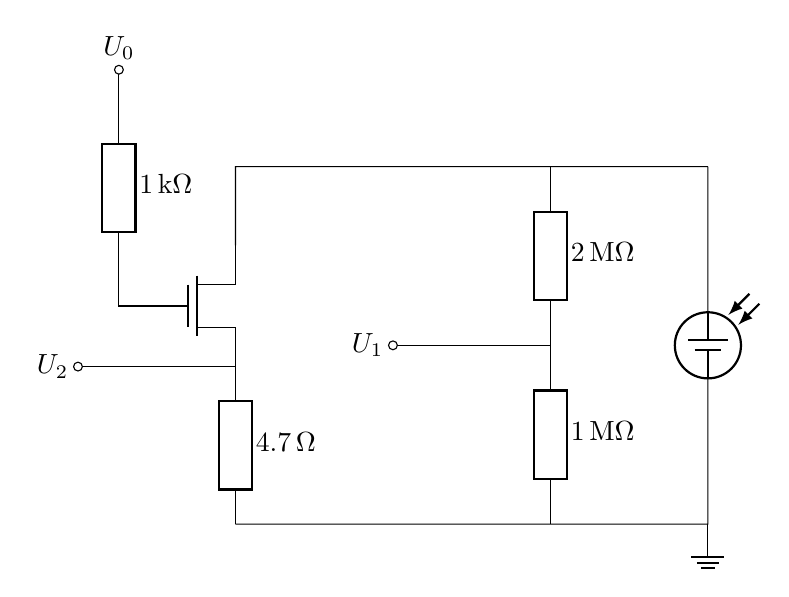
\begin{tikzpicture}[scale=2]
  \draw (0, 0) node[nmos] (mosfet) {};
  \draw (mosfet.G) to[short] ++(-.25, 0) to[R, l_={1<\kilo\ohm>},-o] ++(0, 1.5) node[above] {$U_0$};
  \draw (mosfet.S) to[short,-o] ++(-1, 0) node[left] {$U_2$};
  \draw (mosfet.S) to[R={4.7<\ohm>}] ++(0, -1) coordinate (shuntground);
  \draw (mosfet.D) to[short] ++(0, .5) to[short] ++(2, 0) coordinate (R2) to[short] ++(1, 0) coordinate (PV+);
  \draw (shuntground) to[short] ++(2, 0) coordinate (R1) to[short] ++(1, 0) node (PV-) [ground] {} to[pvsource] (PV+);
  \draw (R2) to[R={2<\mega\ohm>}] ($(R2)!.5!(R1)$) to[R={1<\mega\ohm>}] (R1);
  \draw ($(R2)!.5!(R1)$) to[short,-o] ++(-1, 0) node[left] {$U_1$};
\end{tikzpicture}
\end{document}